\documentclass{article}
\usepackage[letterpaper]{geometry}
\usepackage{graphicx}
\graphicspath{{./img/}}
\title{2411 HW 5}
\author{Duncan Wilkie}
\date{8 October 2021}

\begin{document}

\maketitle

\section{}
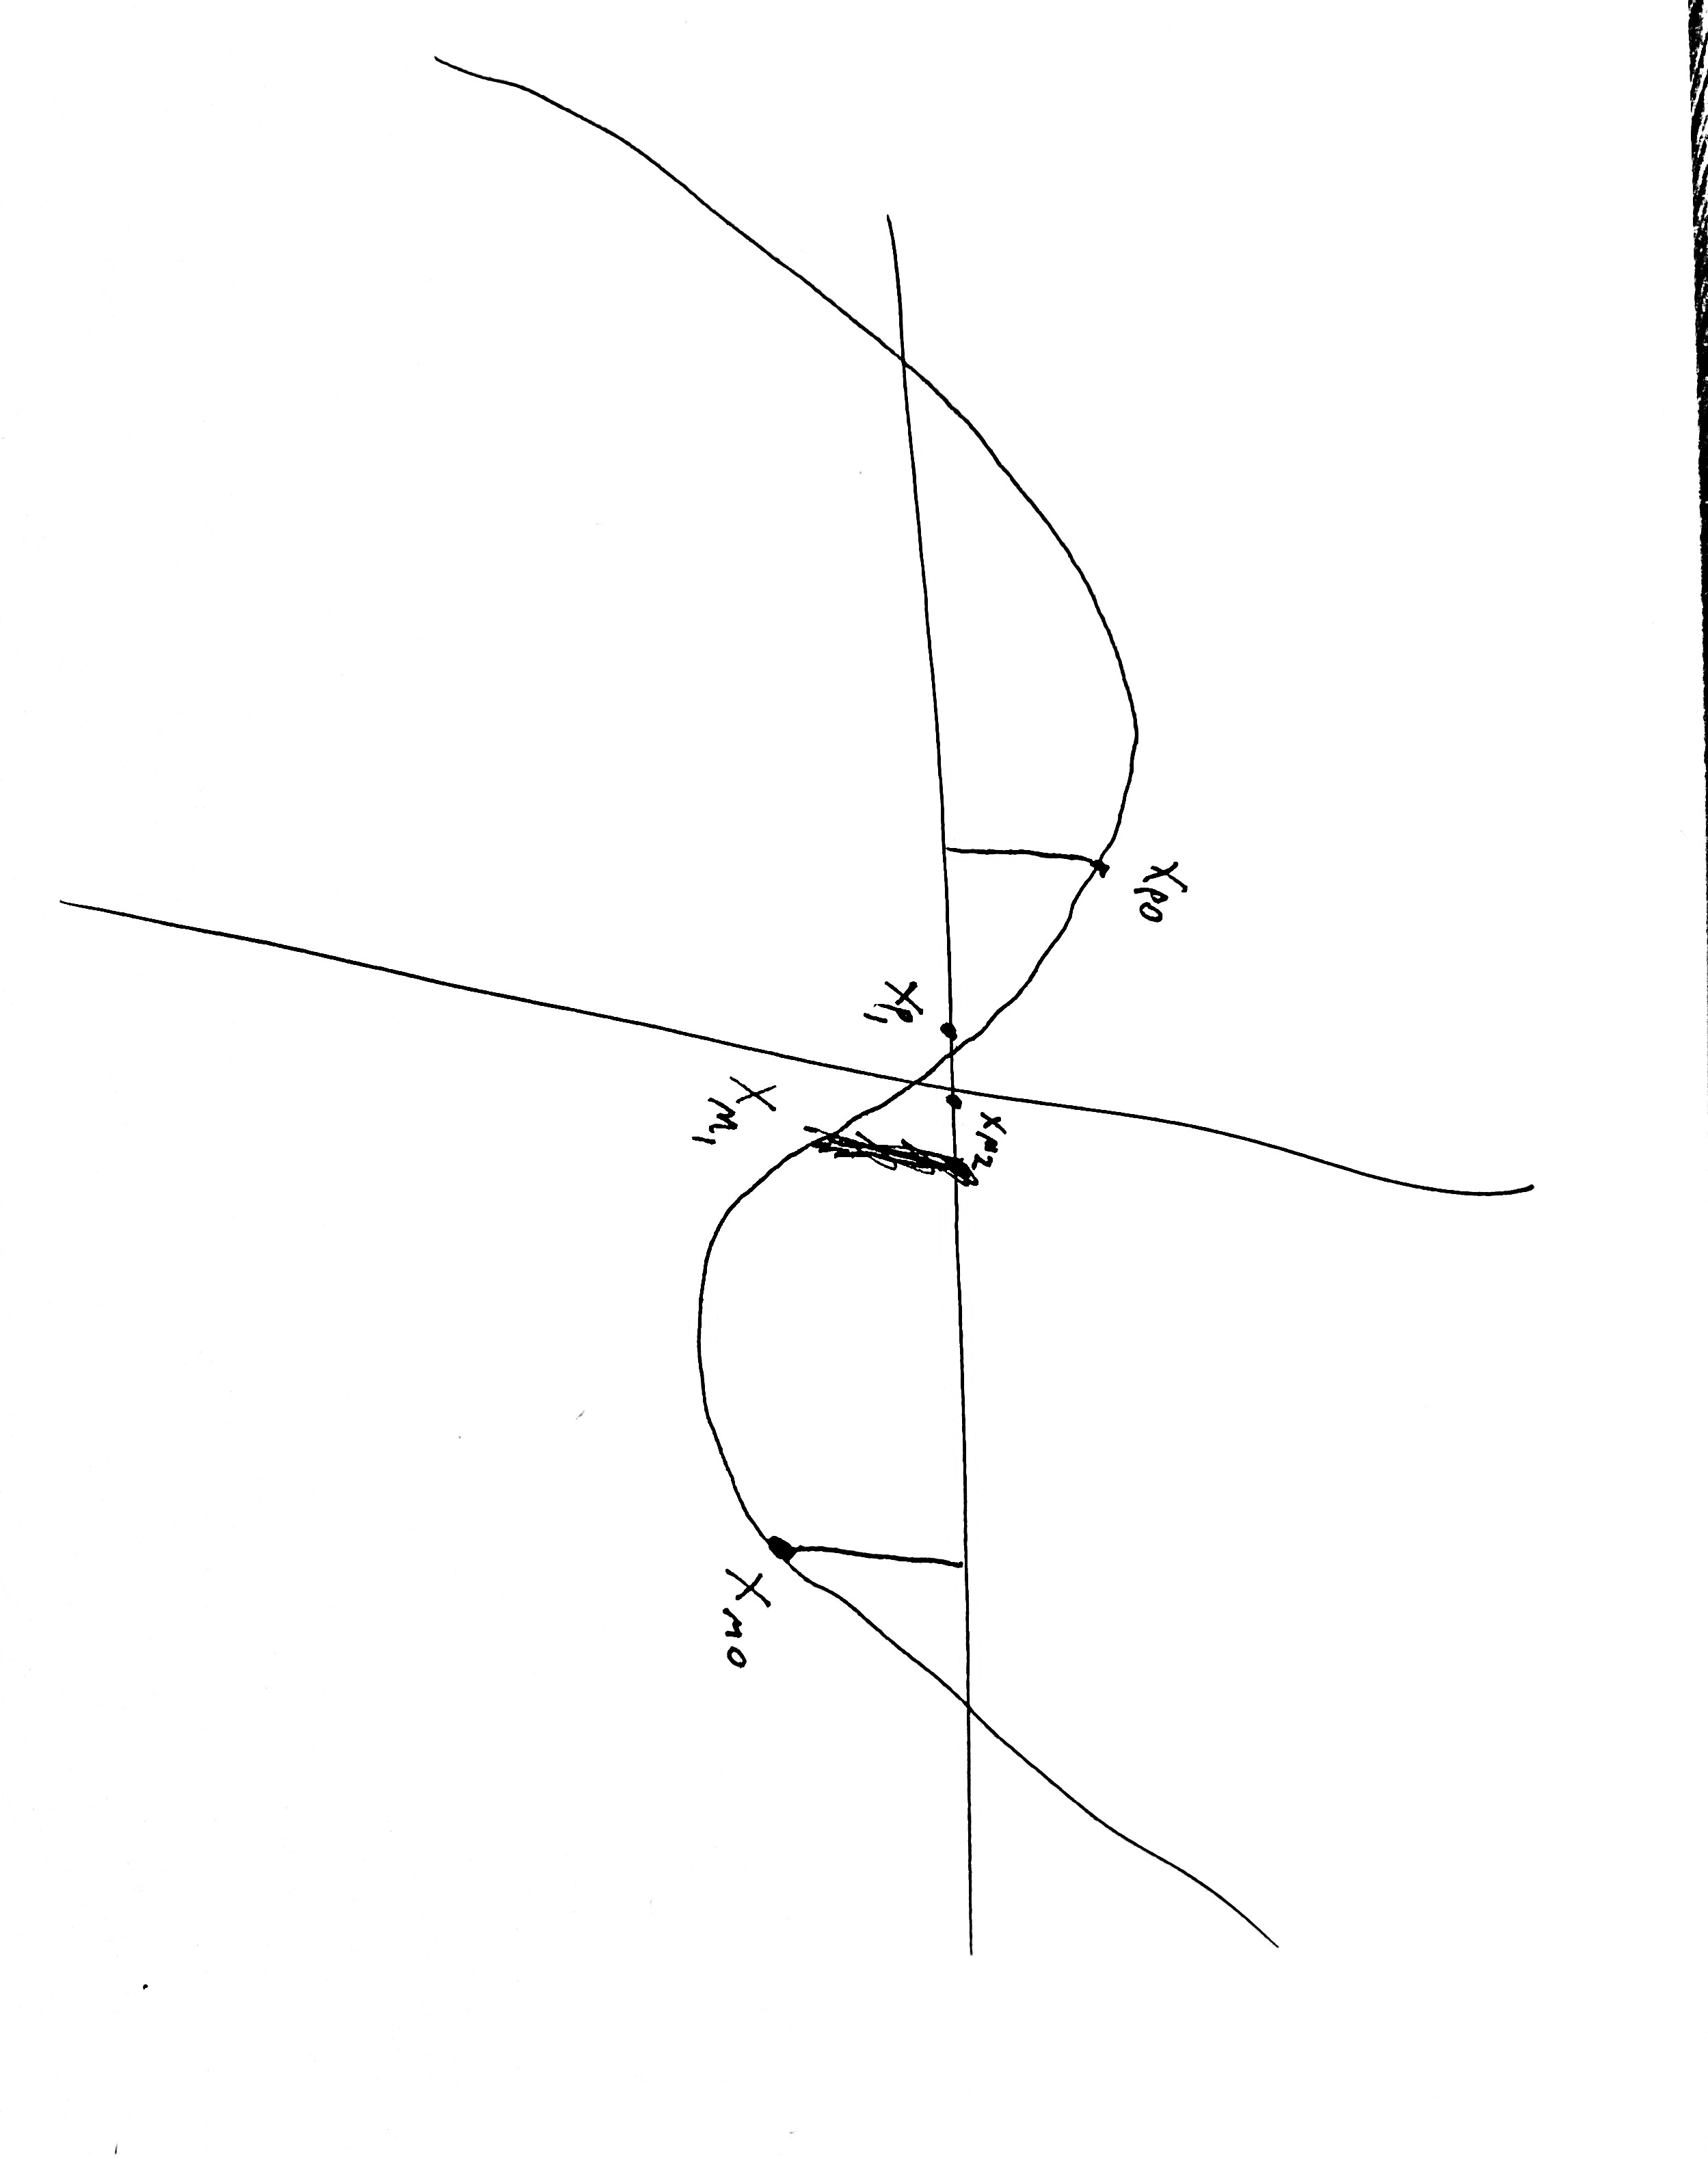
\includegraphics[scale = 0.1, angle=90]{p1.jpg}
\section{}
The program appears in the Script Files section.
\newpage
\section{Script Files}
\begin{verbatim}
#include <iostream>
#include <cmath>

using namespace std;

float f(double x) {
  return 5 / 2 * pow(x, 3) - 3 / 2 * x;
}

int main() {
  float h = 0.1, xm = -1, xp = xm + h, xmid, fmid;

  cout << "xp xm fmid" << endl;
  while ((f(xm) * f(xp) >= 0.0f)) {
    xp += h;
  }

  for (int i = 0; i < 20; i++) {
    xmid = (xm + xp) / 2;
    fmid = f(xmid);

    cout << xp << " " << xm << " " << fmid  << endl;

    if (abs(fmid) < 1E-6) break;

    if (!(f(xm) * fmid >= 0.0f)) {
      xp = xmid;
    }

    if (!(f(xp) * fmid >= 0.0f)) {
      xm = xmid;
    }

  }

  return 0;

}
\end{verbatim}



\end{document}
%%% Local Variables:
%%% mode: latex
%%% TeX-master: t
%%% End:
